

\section{Face Classification}

\label{sec:classification}


We traverse each face of the primitives, and determine which belong to the final mesh. The faces are classified by evaluating their inclusion label vector. Our classification method utilizes the space coherence of the label vectors, and shares the classification results among neighboring faces. Because we store the neighboring faces in the edges where intersections occur, the difference of labels between adjacent faces are computed according to the BSP constructed with these neighboring faces. For arbitrary adjacent faces $\bm{s}_1$ and $\bm{s}_2$, the label vectors $\bm{\Lambda}(\bm{s}_1)$ and $\bm{\Lambda}(\bm{s}_2)$ differ if their shared edge $\bm{e}_{12}$ lies on the surface of any other primitive.
In that cases, some neighboring faces should be stored on $\bm{e}_{12}$. The owner primitives of these neighboring faces indicate which labels differ. If there are neighboring faces from mesh $M_x$, the labels $\lambda_x(\bm{s}_1)$ and $\lambda_x(\bm{s}_2)$ differ. We outline our classification method in Algorithm \ref{code:floodfill}.

\begin{algorithm}[ht]
\caption{Fast Face Classification}
\label{code:floodfill}
\textbf{Input: } Tessellated primitives and boolean expression $f$

\textbf{Output: } Classification $f(\bm{\Lambda}(\bm{s}_i))$ of each face $\bm{s}_i$


\begin{algorithmic}[1]
\State Select a proper seed face $\bm{s}_0$
\State Compute the seed label vector $\boldsymbol{\Lambda}(\bm{s}_0)$
\State \Call{propagate} { $\bm{s}_0$ , $\boldsymbol{\Lambda}(\bm{s}_0)$}
\State
\Function{propagate}{ $\bm{s}$ , $\boldsymbol{\Lambda}(\bm{s})$}
    \State Compute $f(\boldsymbol{\Lambda}(\bm{s}))$
    \For {each neighboring face $\bm{s}_{s, i}$}
        \If {$\bm{s}_i$ has been classified}
            \State continue
        \EndIf
        \If {there are PBI-reps ${\bm{\mathcal{I}}}_k$ on $\bm{e}(\bm{s}_{s, i}, s)$}
            \State compute $\boldsymbol{\Lambda}(\bm{s}_{s, i})$ by $\boldsymbol{\Lambda}(\bm{s})$ and ${\bm{\mathcal{I}}}_k$
            \State \Call{propagate} { $\bm{s}_{s, i}$ , $\boldsymbol{\Lambda}(\bm{s}_{s, i})$}
        \Else
            \State \Call{propagate} { $\bm{s}_{s, i}$ , $\boldsymbol{\Lambda}(\bm{s})$}
        \EndIf
    \EndFor
\EndFunction
\end{algorithmic}
\end{algorithm}


\subsection{Label Computation}
\label{sec:propagation}

In methods like \cite{feito2013fast,ogayar2015deferred}, the face barycenter is used to compute the inclusion label of the face. This is because the face can be classified as a whole, and all inner points of the face has the same label vector. In methods like \cite{zhou2016mesh}, points inside the cell is used for label computation, and the face labels are decided by the labels of the two sides of the face. However, all these methods require to construct new vertices, whose coordinates require rational numbers to store, or round-off errors may be introduced. Incorrect label computation may occur because of such errors. To avoid this, we use the vertices instead, the exact coordinates of which are known.

\begin{wrapfigure}{r}[0in]{0in}
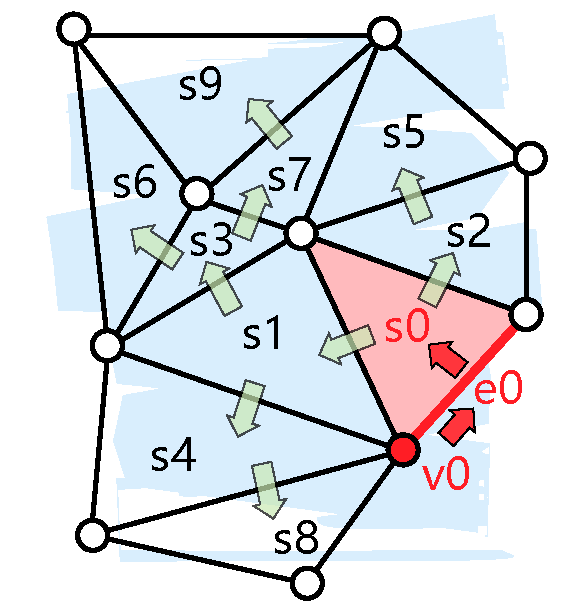
\includegraphics[width=1.3 in]{propagate}
\end{wrapfigure}


However, there are two discrepancies between the face labels and vertex labels. First, the vertex label is not always equal to the face label. Second, the face label has two subclasses in the $on$ case, $same$ and $oppo$, because the face has an orientation.

To deal with these discrepancies, we start from a seed vertex $\bm{v}_0$, which is one of the end point of an edge $\bm{e}_0$ of a face $\bm{s}_0$. We assume that the label vector $\bm{\Lambda}(\bm{v}_0)$ is known.
Then we use $\bm{\Lambda}(\bm{v}_0)$ to compute $\bm{\Lambda}(\bm{e}_0)$, and then $\bm{\Lambda}(\bm{s}_0)$. The trace of label propagation is:
\begin{equation}
\bm{v}_0\to \bm{e}_0\to \bm{s}_0\to \bm{s}_1\to \bm{s}_2\to ...~~~,
\end{equation}
There are three basic operations: $\bm{v}_{\bm{e}}\to \bm{e}$, $\bm{e}_{\bm{s}}\to \bm{s}$ and $\bm{s}_i\to \bm{s}_j$, where $\bm{v}_{\bm{e}}$ is the end point of $\bm{e}$,
$\bm{s}_{\bm{s}}$ is the edge of $\bm{s}$,
and $\bm{s}_i$ is adjacent to $\bm{s}_j$.

\begin{theorem}
  \label{thm:porder}
  Given the partial orders $on \succ in$ and $on \succ out$, the following relationship is true for labels within the tessellated primitives:
  \begin{equation}
    \lambda_k(\bm{v}_{\bm{e}_{\bm{s}}}) \succeq \lambda_k(\bm{e}_{\bm{s}}) \succeq \lambda_k(\bm{s}),
  \end{equation}
  where $\lambda_k(x)$ is the label of $x$ for a certain primitive $M_k$.
\end{theorem}

\begin{proof}
We prove this theorem by contradiction. When $\lambda_k(\bm{v}_{\bm{e}_{\bm{s}}}) \succeq \lambda_k(\bm{e}_{\bm{s}})$ is not satisfied, it means for a certain label $\lambda_k$, $\lambda_k(\bm{v}_{\bm{e}_{\bm{s}}})$ is $in$ or $out$, but $\lambda_k(\bm{e}_{\bm{s}}) \neq \lambda_k(\bm{v}_{\bm{e}_{\bm{s}}})$.
Let us assume that $\lambda_k(\bm{v}_{\bm{e}_{\bm{s}}})=in$ and $\lambda_k(\bm{e}_{\bm{s}})=on$ or $out$.

Because $\bm{v}_{\bm{e}_{\bm{s}}}$ is inside of closed regular set (solid) $M_k$, according to the continuity of space, any point in $U(\bm{v}_{\bm{e}_{\bm{s}}})$, which is the neighborhood of $\bm{v}_{\bm{e}_{\bm{s}}}$, should be inside of $M_k$.
And because $\bm{e}_{\bm{s}}^{\circ}\cap U(\bm{v}_{\bm{e}_{\bm{s}}})$ is not empty (superscript $\circ$ means interior), $\bm{e}_{\bm{s}}$ should be inside of $M_k$, which contradict our assumption.
\end{proof}

It indicates that when we perform $\bm{v}_{\bm{e}}\to \bm{e}$ and $\bm{e}_{\bm{s}}\to \bm{s}$, from a low-dimension to a high-dimension, we decide whether the $on$ label changes to $in$ or $out$, or remains $on$.
In addition, when considering the orientation of the face, we also need to determine whether the $on$ labels change to $same$ or $oppo$ during the $\bm{e}_{\bm{s}}\to \bm{s}$ operation.


\begin{figure}[t]
\centering
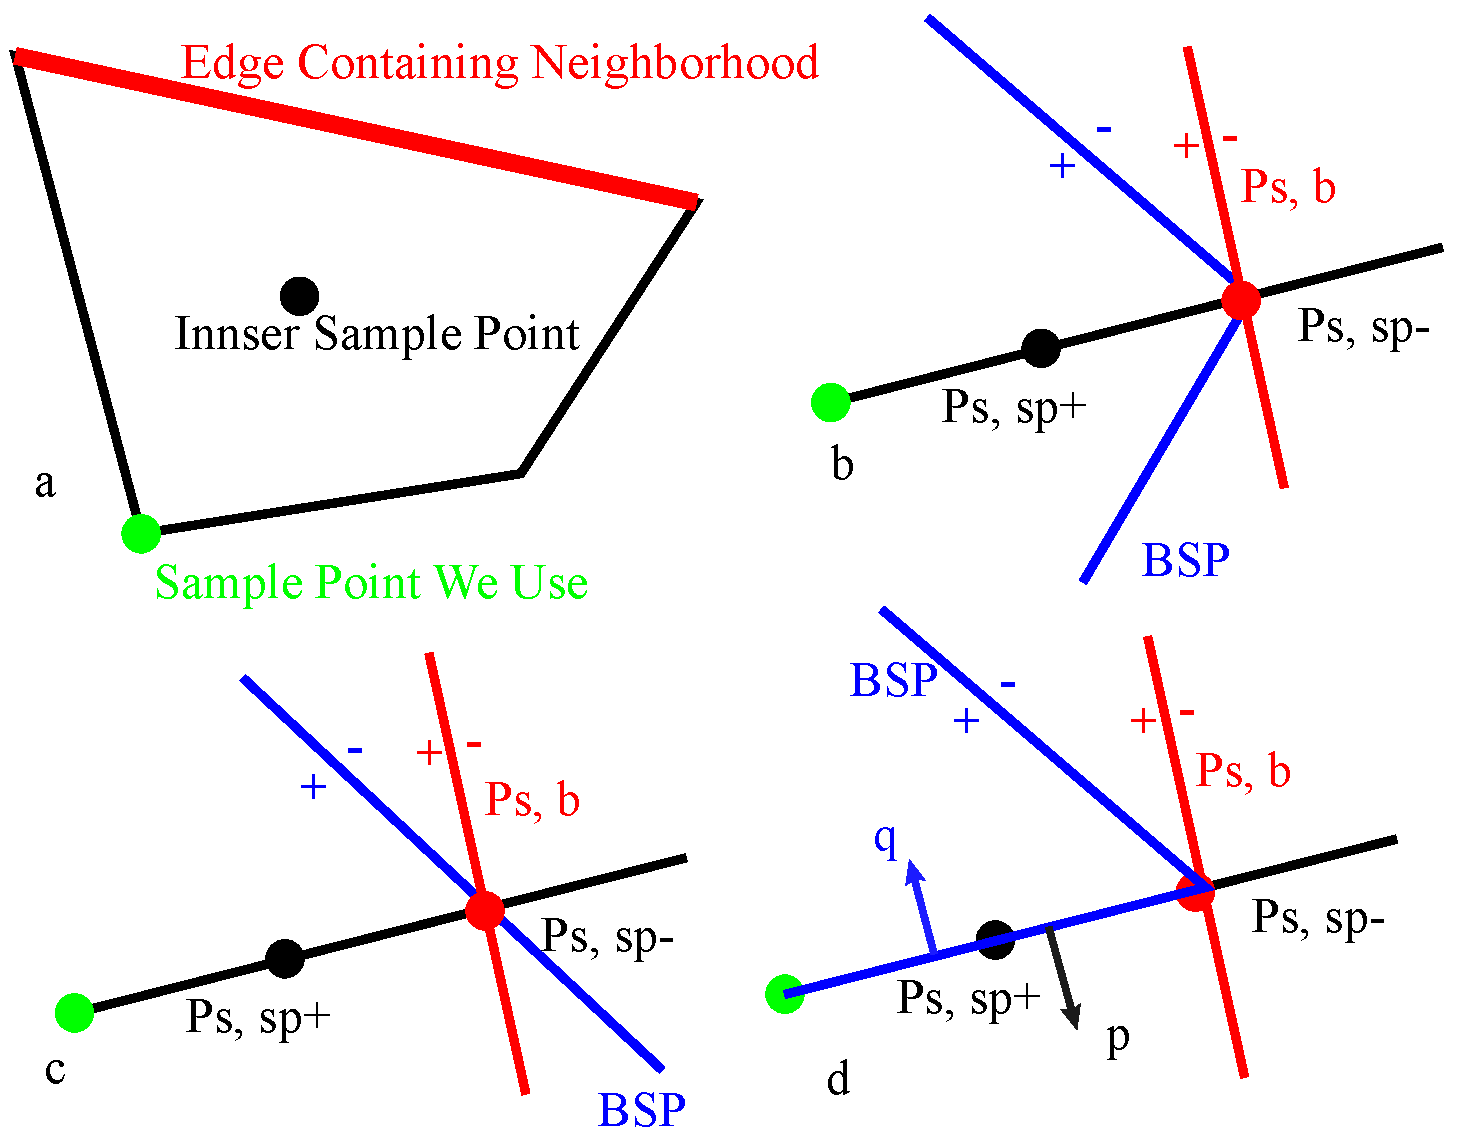
\includegraphics[width=3in]{bsps}
\caption{a) Because the inner sample point includes geometric constructions, we choose the face vertex (orange) instead to compute the face label. b-d) Different types of classification. The simple structure of the neighborhood BSP guarantees the same classification result for all of the points on $\bm{p}_{\bm{s}, sp}^+$. In d), the classification result is $on$ so it is necessary to determine the orientation from the normal of the BSP splitting plane $q$ and the face normal $p$. In this cases, the label should be $oppo$ because $p$ and $q$ are opposite.}
\label{fig:bsps}
\end{figure}

\vspace{0.5em}
\noindent\textbf{$\bm{\bm{e}_{\bm{s}}\to \bm{s}}$: } From theorem \ref{thm:porder}, we know that if $\lambda_k(\bm{e}_{\bm{s}}) \neq on$, then $\lambda_k(\bm{e}_{\bm{s}})=\lambda_k(\bm{s})$.
Conversely, when $\lambda_k(\bm{e}_{\bm{s}}) = on$, we can build a trivial BSP \cite{thibault1987set} using these the neighboring faces which belongs to $M_k$ stored in $\bm{e}_{\bm{s}}$.
The BSP can be used to compute inclusion state $\lambda_k(\bm{s})$ if a point can be sampled from $\bm{s}^{\circ} \cap \bm{U}(\bm{e}_{\bm{s}})$, where $\bm{U}(\bm{e}_{\bm{s}})$ is the neighborhood space of $\bm{e}_{\bm{s}}$. However, we cannot guarantee that such a point can be found with exact representation of double-precision.

\begin{theorem}
  \label{thm:bsp}
  The BSP is constructed by the neighboring faces around a certain edge $\bm{e}$. Then the inclusion states of all the points on interior of the half plane $\bm{h}$ are the same, if 1) $\bm{e}$ is within $\bm{h}$, and 2) $\bm{e}$ is the boundary of $\bm{h}$.
\end{theorem}
\begin{proof}
  The correctness of the theorem is obvious because the supporting planes of the neighboring faces always cross the edge $\bm{e}$ and extend to infinity.
\end{proof}

Let $\bm{h}_{\bm{s}}^+$ be the half of the supporting plane of $\bm{s}$ which lies on the interior side of $\bm{e}_{\bm{s}}$ (see Fig. \ref{fig:bsps}). By theorem \ref{thm:bsp}, the label of points on the half plane $\bm{h}_{\bm{s}}^+$ are identical.
Since $\bm{h}_{\bm{s}}^+ \cap \bm{s} \neq \varnothing$, we can compute $\lambda_k(\bm{s})$ by determining $\lambda_k(\bm{v}_x)$, where the vertex $\bm{v}_x \in \bm{h}_{\bm{s}}^+$. For polygons, we can always find at least one such vertex, which is represented exactly (by planes or vertex coordinates). In addition, we assign each BSP splitting plane a normal vector by the normal of the triangle it contains, from which we can decide the orientation ($same$ or $oppo$) when $\lambda_k(\bm{s})=on$.


\vspace{0.5em}
\begin{wrapfigure}{r}[0in]{0in}
 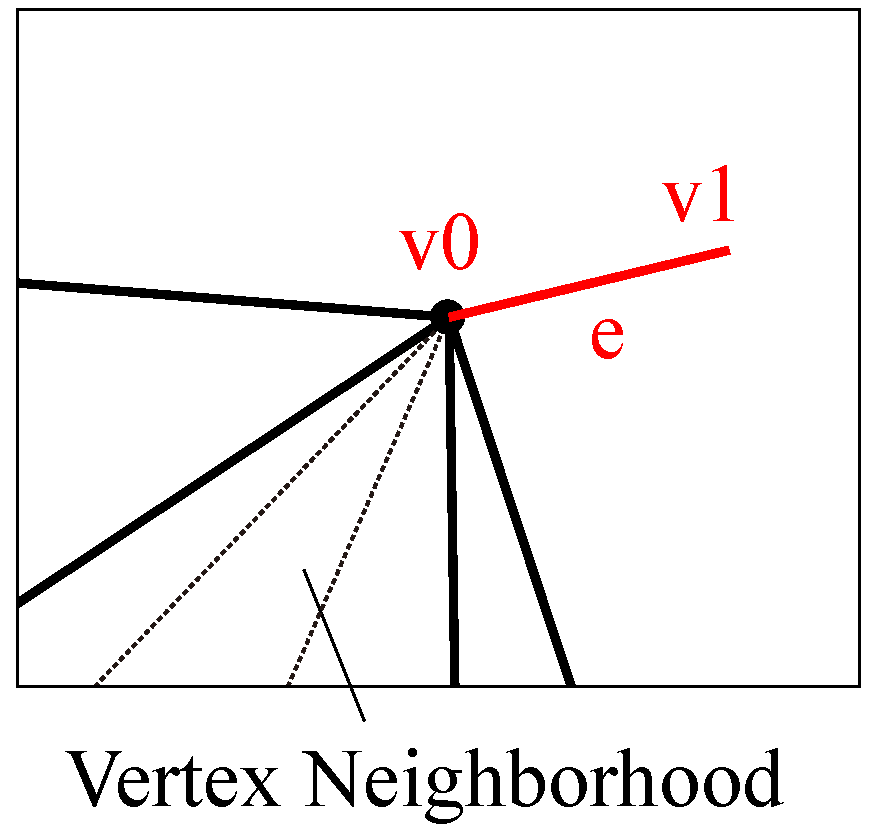
\includegraphics[width=1.3 in]{vneighbor}
\end{wrapfigure}
\noindent\textbf{$\bm{\bm{v}_{\bm{e}}\to e}$: }If $\lambda_k(\bm{v}_{\bm{e}})=on$, we first check whether $\lambda_k(\bm{e}) = on$, by checking whether there is neighboring faces from $M_k$ on $\bm{e}$. If not, we need to find where $\bm{v}_{\bm{e}}$ lies on $M_k$.
Because our tessellated meshes contain connectivity information, we can easily find all neighboring faces of $\bm{v}_{\bm{e}}$.
After that, the similar BSP-based classification method (as in ${\bm{e}_{\bm{s}}\to \bm{s}}$) can be used to determine the high dimension label $\lambda_k(\bm{e})$. We use the other end point $\bm{v}'_{\bm{e}}$ as the sample point for the BSP classification.


\vspace{0.5em}
\noindent\textbf{$\bm{s}_i\to \bm{s}_j$: } We need to determine which labels change if shared edge contains neighboring faces from other primitives. We can know which labels differ by the owner primitives of these neighboring faces. And the recomputation of these labels is exactly the same as in $\bm{\bm{e}_{\bm{s}}\to \bm{s}}$.


\subsection{Acceleration by Caching}
\label{sec:acc}


If the CSG tree is large, with hundreds of primitive nodes, evaluations of boolean expression by inclusion label vectors of each face can be costly. However, using label space coherence, we can reduce the computation time by caching the evaluation results.


The basic caching strategy is to cache the final evaluation results. Faces which share the same label vector can be classified together. We can also perform an intermediate results cache. The boolean expression can be simplified if some components of label vector are known. For example, assume we have a boolean expression $f = M_1\cup (M_2\cap M_3-M_4)$. Given the values of two labels $\lambda_1(\bm{s}_i)=out$, $\lambda_2(\bm{s}_i)=in$, the expression can be rewritten as $f(\lambda_1=out, \lambda_2=in)=out\cup (in\cap M_3-M_4)$. Using the combination rules, we can simplify the expression to $f(\lambda_1=out, \lambda_2=in)=M_3-M_4$.
In a large CSG, a certain primitive often intersects with only a few other primitives $\Theta= \{M_{n_1}, M_{n_2}, \cdots, M_{n_x}\}$. All of the faces in this primitive have the same labels with respect to primitives not in $\Theta$. Therefore, if we can determine these fixed labels and simplify the boolean function, then we compute the final label in this primitive based on the simplified expression.


\iffalse
\subsection{Tessellating on Classification}
We find for a CSG with many meshes, a large percentage of intersections are invalid (see \S\ref{sec:degenerate} for 'invalid'). Tessellation according to these invalid intersections is not necessary. To avoid unnecessary tessellation, we can give an early prediction of which intersections are invalid by intersections information of faces, but have to embed the tessellation stage into the classification stage, which we call it 'tessellating on classification'.

In most situations, a certain faces $\bm{s}$ only intersect with a few other meshes $\Theta(\bm{s})$. We can use the same cache strategy in \S\ref{sec:acc} to shrink the original CSG into a smaller one by the common labels of $\{P_i\}\backslash\Theta(\bm{s})$, where $\{P_i\}$ means all the primitive meshes. After the shrinking, the primitive meshes of the CSG must be from $\Theta(\bm{s})$. If any mesh in $\Theta(\bm{s})$ does not appear in the shrinked CSG, it means the label of that mesh does not change the classification result, which in another word, intersections on $\bm{s}$ from that mesh are invalid and do not affect the classification of any subfaces of $\bm{s}$. If the shrinked CSG is trivial which does not contain any primitives, it means $\bm{s}$ does not need tessellation. In this way, we save the computation time, and simplify the topology of the final result mesh. Because we can only shrink the CSG for $\bm{s}$ when we classify it---before that the labels of meshes from $\{P_i\}\backslash\Theta(\bm{s})$ are not known---we do not perform tessellation until we do the classification.
\fi
